\documentclass[12pt, a4paper, oneside]{ctexart}
\usepackage{amsmath, amsthm, amssymb, appendix, bm, graphicx, hyperref, mathrsfs,adjustbox}
\usepackage{enumerate}
\title{\textbf{论文标题}}
\author{tanghongyu}
\date{\today}
\linespread{1.5}
\newtheorem{theorem}{定理}[section]
\newtheorem{definition}[theorem]{定义}
\newtheorem{lemma}[theorem]{引理}
\newtheorem{corollary}[theorem]{推论}
\newtheorem{example}[theorem]{例}
\newtheorem{proposition}[theorem]{命题}
\renewcommand{\abstractname}{\Large\textbf{摘要}}

\begin{document}

\maketitle

\setcounter{page}{0}
\maketitle
\thispagestyle{empty}
\newpage
\begin{abstract}
    这里是摘要。这里是摘要。这里是摘要。这里是摘要。这里是摘要。这里是摘要。这里是摘要。这里是摘要。这里是摘要。这里是摘要。这里是摘要。这里是摘要。
    \par\textbf{关键词:}这里是关键词; 这里是关键词.
\end{abstract}

\newpage
\pagenumbering{Roman}
\setcounter{page}{1}
\tableofcontents
\newpage
\setcounter{page}{1}
\pagenumbering{arabic}

\section{定理}

%\subsection{二级标题}






\section{表格}

\begin{table}[htbp]
    \centering  % 显示位置为中间
    \caption{ }  % 表格标题
    \label{tab1}  % 用于索引表格的标签
    %字母的个数对应列数,|代表分割线
    % l代表左对齐,c代表居中,r代表右对齐
    \begin{tabular}{|c|c|c|}
    \end{tabular}
\end{table}
%\begin{theorem}

%\end{theorem}

\begin{table}[htbp]
    \centering  % 显示位置为中间
    \caption{ }  % 表格标题
    \label{tab2}  % 用于索引表格的标签
    %字母的个数对应列数,|代表分割线
    % l代表左对齐,c代表居中,r代表右对齐
    \begin{adjustbox}{max width=\textwidth}
        \begin{tabular}{|c|c|c|}
        \end{tabular}
    \end{adjustbox}
\end{table}
\begin{table}[htbp]
    \centering  % 显示位置为中间
    \caption{ }  % 表格标题
    \label{tab111}  % 用于索引表格的标签
    %字母的个数对应列数,|代表分割线
    % l代表左对齐,c代表居中,r代表右对齐
    \begin{tabular}{|c|c|}
    \end{tabular}
\end{table}


\begin{table}[htbp]
    \centering  % 显示位置为中间
    \caption{ }  % 表格标题
    \label{tab333}  % 用于索引表格的标签
    %字母的个数对应列数,|代表分割线
    % l代表左对齐,c代表居中,r代表右对齐
    \begin{tabular}{|c|c|}
    \end{tabular}
\end{table}

\begin{table}[htbp]
    \centering  % 显示位置为中间
    \caption{ }  % 表格标题
    \label{tab222}  % 用于索引表格的标签
    %字母的个数对应列数,|代表分割线
    % l代表左对齐,c代表居中,r代表右对齐
    \begin{tabular}{|c|c|}
    \end{tabular}
\end{table}


\section{图片}
\subsection{单图}
\begin{figure*} [htbp!]
    \centering
    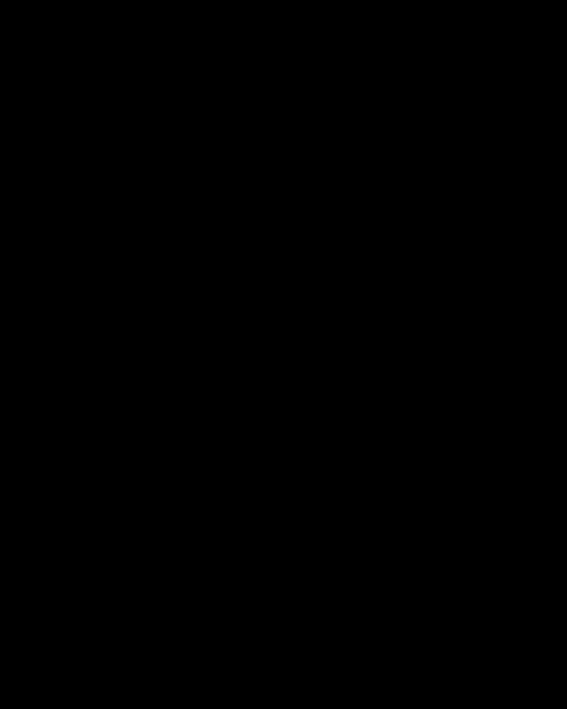
\includegraphics[scale=0.5]{fig.png}
    \caption{图1}
    \label{fig1}
\end{figure*}
\subsection{多图}
\newpage

\section{公式}
\subsection{单行公式}
单行公式较为简单,直接在\$...\$之间输入公式代码即可,例如:\par
\begin{equation}
    E_0=mc^2
\end{equation}

\subsection{多行公式}
多行公式涉及到手动在恰当的地方用$\backslash$$\backslash$分行,
同时用\&对齐,本模板中以等号对齐为例:\\
\begin{equation}
    \begin{split}
        Dec_{sk}(\alpha)&=(a_1\cdot a_2)+(a_2\cdot b_1)+(a_1\cdot b_2)\\
        &= m_1m_2-m_1b_2-m_2b_1+b_1b_2+m_2b_1-b_1b_2+m_1b_2-b_1b_2\\
        &= m_1m_2-b_1b_2
    \end{split}
\end{equation}
\subsection{分情况讨论}

$$
    \begin{cases}
        \Delta >0 & \text{方程有两个不相等的实根} \\
        \Delta =0 & \text{方程有两个相等的实根}  \\
        \Delta <0 & \text{方程有两个复根}     \\
    \end{cases}
$$
\subsection{公式编号}
还没想好捏


\newpage
\begin{thebibliography}{99}
    \bibitem{a}作者. \emph{文献}[M]. 地点:出版社,年份.
    \bibitem{b}作者. \emph{文献}[M]. 地点:出版社,年份.
\end{thebibliography}

\begin{appendices}
    \renewcommand{\thesection}{\Alph{section}}
    \section{附录标题}
    这里是附录.
\end{appendices}

\end{document}